\chapter{Requirements analysis}
\section*{Introduction}
In this section, we will present the background study of our project in order to identify the
actors who will interact with the system and to list the functional requirements and the non 
functional requirements as well as  our project's backlog and plan our sprints 

\section{Functional requirements}
In the following we will describe the functional requirements of our future system which we will
During this internship, we plan to carry out 
\begin{itemize}
    \item \texbf{Manage system configuration :} The administrator must be able change system configurations (Policies, Visas ..ect)
    \item \texbf{Manage profiles :} The user must be able to change his profile information
    \item \texbf{Create travel orders :} The user must be able to create travel order drafts
    \item \texbf{Manage travel orders :} The agent must be able to change travel orders' status and add attachments 
    \item \texbf{Confirm travel orders :}The manager must be able to confirm travel order drafts and validate the agent's work
\end{itemize}

\section{Non functional requirements}
Apart from the functional requirements that our future system must provide, there is also a
set of non-functional constraints to be respected that represents a desired property of the
system.
Among these requirements are the following: 
\begin{itemize}
\item \textbf{Scalability:} the system must respect a modular architecture where each module
must respond to a set of functionalities covering a common need in order to
to facilitate its reusability for future needs and thus ensure the scalability of the
system
\item \textbf{Security:} our future product must provide a system of restriction on the
manipulations not authorized to a user group with a role defined on the
system
\item \textbf{Internationalization:} our application must have the option of adding more languages
\end{itemize}
\section{Identification of actors}
The system is intended to be used by different users grouped into different profiles:
\begin{itemize}
    \item \textbf{Administrator : }Manages accounts and system configurations
    \item \textbf{User : }Edits his profile and submit travel orders
    \item \textbf{Manager : }Confirm and validate travel orders
    \item \textbf{Agent : }Add reservations to travel orders
\end{itemize}
\section{Project management with Scrum}
   Having opted for Agile SCRUM as our methodology we need to define all actors that take part in the project analysis and implementation and their responsibilities.

\begin{table}[H]
\caption{ Scrum Team }
\begin{tabular}{|p{4,5cm}|p{5,25cm}|p{5,25cm}|}
\hline
\textbf{Role} 
&\textbf{Responsibilities}
&\textbf{Actor}\\
\hline

\hline 
\textbf{- Product Owner} 
&- Identifying core project features\newline{}- Keeping the backlog up-to-date and in priority order\newline{}
&- Amira Hasnaoui\\
\hline

\hline
\textbf{- SCRUM Team} 
&- Modeling\newline{}- Tests and validation\newline{}- Development\newline{}
&- Mohammed Amine ElAmri\\
\hline

\hline
\textbf{- SCRUM Master} 
&- Identify needs and requirments\newline{}- Setup meetings and deadlines
&- Amira Hasnaoui\\
\hline



\end{tabular}
\end{table}
     


	\section{Global project backlog}
	In the following we will present our Product Backlog which will contain the list of
expected system functionality estimate in time and plan according to required priorities
by our Product Owner 
\begin{center}
\begin{longtable}{|p{0.5cm}|p{3.5cm}|p{6,5cm}|p{2cm}|p{2cm}|}
\caption{ Project backlog }
\hline
\textbf{ID} 
&\textbf{Theme}
&\textbf{User Story}
&\textbf{Estimation}
&\textbf{Priority}\\
\hline
1
&Authentification
&As an Administrator , Agent , Manager or User, I want to be able to log-in
&12h
&HIGH
\hline

2
&\multirow{4}{*}{\begin{tabular}[c]{@{}l@{}}Account Managment\end{tabular}}
&As an Administrator, I want to be able to create user accounts
&8h
&HIGH\\ \cline{1-1} \cline{3-5} 

3
&
&As an Administrator, I want to be able to edit user details
&4h
&LOW\\
\cline{1-1} \cline{3-5} 
4
&
&As a Manager, I want to be able to edit user roles
&4h
&LOW\\
\cline{1-1} \cline{3-5} 
5
&
&As an Administrator, I want to be able to view the users list
&10h
&MEDIUM\\
\hline
6
&\multirow{2}{*}{\begin{tabular}[c]{@{}l@{}}Profile Managment\end{tabular}}
&As a User , I want to be able to view my profile details
&8h
&HIGH\\
\cline{1-1} \cline{3-5} 
7
&
&As a User , I want to be able to change my profile details
&2h
&LOW\\
\hline
8
&\multirow{11}{*}{\begin{tabular}[c]{@{}l@{}}Configuration\end{tabular}}
&As an Administrator , I want to be able to view, create, edit, delete and import new countries
&16h
&HIGH\\
\cline{1-1} \cline{3-5} 
9
&
&As an Administrator , I want to be able to view, create, edit, delete and import flight policies
&8h
&MEDIUM\\
\cline{1-1} \cline{3-5} 
10
&
&As an Administrator , I want to be able to view, create, edit, delete and import hotel reservation policy
&8h
&MEDIUM\\
\cline{1-1} \cline{3-5} 
11
&
&As an Administrator , I want to be able to view, create, edit, delete and import per diem policy
&8h
&MEDIUM\\
\cline{1-1} \cline{3-5} 
12
&
&As an Administrator , I want to be able to view, create, edit, delete and import visa models
&6h
&LOW\\
\cline{1-1} \cline{3-5} 
13
&
&As an Administrator , I want to be able to view, create, edit, delete and import vaccins
&6h
&LOW\\
\cline{1-1} \cline{3-5} 
14
&
&As an Administrator , I want to be able to attribute vaccines to countries
&6h
&LOW\\
\cline{1-1} \cline{3-5} 
15
&
&As an Administrator , I want to be able to attribute visas to countries
&6h
&LOW\\
\cline{1-1} \cline{3-5} 
16
&
&As an Administrator , I want to be able to create , edit and delete administrative grades
&8h
&MEDIUM\\
\cline{1-1} \cline{3-5} 
17
&
&As an Administrator , I want to be to attribute administrative grades to users
&6h
&LOW\\
\cline{1-1} \cline{3-5} 
18
&
&As an Administrator , I want to be able to create , edit and delete mission types
&8h
&LOW\\
\hline
19
&\multirow{10}{*}{\begin{tabular}[c]{@{}l@{}}Travel Order \\Managment\end{tabular}}
&As a User , I want to be able to create , edit and delete travel order drafts
&16h
&HIGH\\
\cline{1-1} \cline{3-5} 
20
&
&As a User , I want to be able to see all my travel orders
&10h
&MEDIUM\\
\cline{1-1} \cline{3-5} 
21
&
&As a User , I want to be able to filter my travel orders by status or date
&6h
&LOW\\
\cline{1-1} \cline{3-5} 
22
&
&As a User , I want to be able to file my travel order drafts and track their progress
&10h
&HIGH\\
\cline{1-1} \cline{3-5} 
23
&
&As an Agent , I want to be able to see all travel orders,
&8h
&MEDIUM\\
\cline{1-1} \cline{3-5} 
24
&
&As an Agent , I want to be able to add attachments to travel orders
&12h
&MEDIUM\\
\cline{1-1} \cline{3-5} 
25
&
&As an Agent , I want to be able to change travel orders' status
&10h
&MEDIUM\\
\cline{1-1} \cline{3-5} 
26
&
&As a Manager , I want to be able to see all travel orders pending my confirmation
&10h
&MEDIUM\\
\cline{1-1} \cline{3-5} 
27
&
&As a Manager , I want to be able to confirm or reject travel orders pending my confirmation
&12h
&MEDIUM\\
\hline
\end{longtable}

\end{center}
    \section{Sprints planning}
    \\Our project lasts three months and follows the Scrum methodology that we have chosen as our working methodology, We can estimate our project on four main phases which are:
    \begin{itemize}
        \item \textbf{Sprint 0 :} Preliminary Phase
        \begin{itemize}
\item Identification of actors
\item Global analysis
\item development environment choices and configuration of the work environment
\item The architectural model
\item Product Backlog
        \end{itemize}
        \item \textbf{Sprint 1 :} Configuration Module
        \begin{itemize}
\item Sprint Backlog 
\item detailed design of the target module
\item Implementation
        \end{itemize}
        \item \textbf{Sprint 2 :} Employee Module
        \begin{itemize}
\item Sprint Backlog 
\item detailed design of the target module
\item Implementation
        \end{itemize}
        \item \textbf{Sprint 3 :} Travel order Module
        \begin{itemize}
\item Sprint Backlog 
\item detailed design of the target module
\item Implementation
        \end{itemize}
    \end{itemize}
    
    \begin{table}[H]
    \begin{tabular}{|p{4cm}|p{6,5cm}|p{4cm}|}
    \hline
\textbf{Sprint} 
&\textbf{User Stories}
&\textbf{Estimation}\\
\hline
Sprint 1
&US1 , US8 , US9 ,  US10 , US11 , US12 , US13 , US14 , US15 , US16 , US17 , US18
&4 weeks\\
\hline
Sprint 2
&US2 , US3 , US4 , US5 , US6 , US7
&3 weeks\\
\hline
Sprint 3
&US19 , US20 , US21 ,  US22 , US23 , US24 , US25 , US26 , US27 
&5 weeks\\
\hline
\end{tabular}
\end{table}


    \section{Project Structure}
    \subsection*{Actors}
    The diagram below helps to highlight the relationships between the different actors
     \begin{figure}[H]
    \begin{center}
        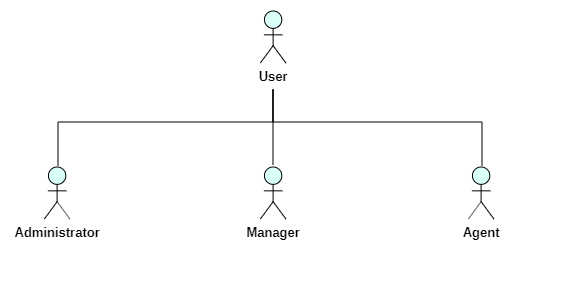
\includegraphics[scale=0.6]{img/actors.png}
        \caption{Actors relationship diagram}
    \end{center}
    \end{figure}
    \subsection*{Global usecase diagram}
    The use case diagram below helps to highlight the relationships between the actors and the system under study
    \begin{figure}[H]
    \begin{center}
        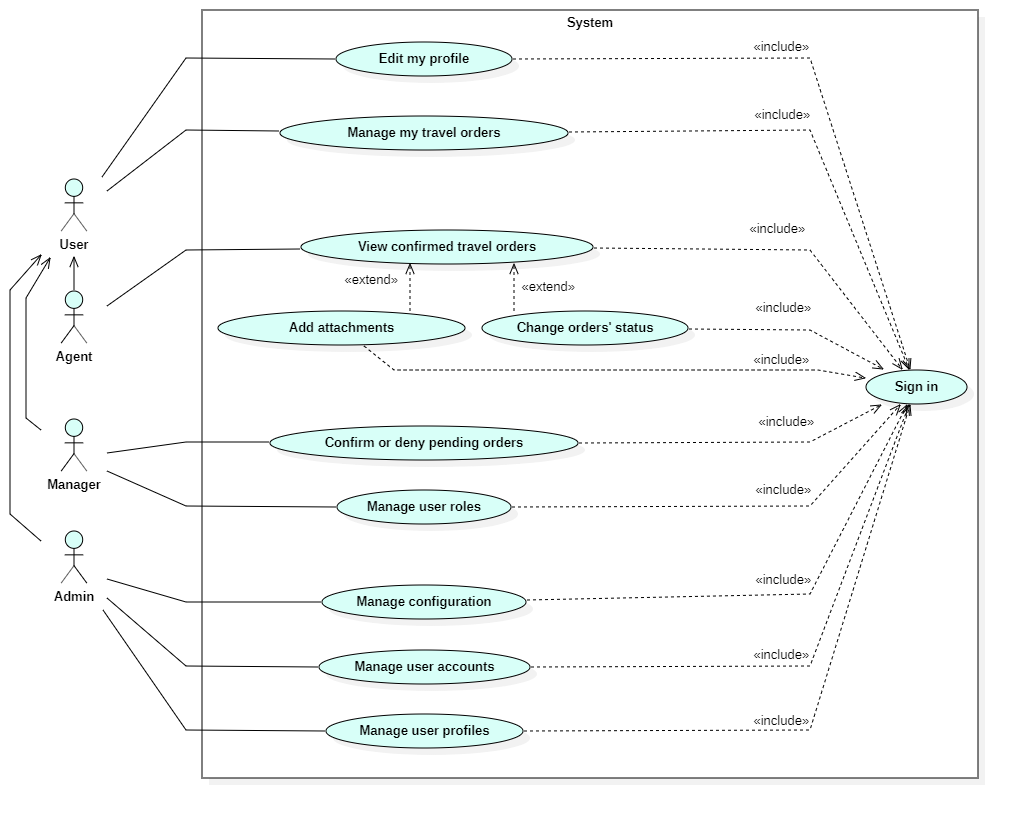
\includegraphics[scale=0.48]{img/global_usecase.png}
        \caption{global use case diagram}
    \end{center}
    \end{figure}
    
\section*{Conclusion}
This chapter summarizes the preliminary study we conducted before entering the development phase of our system. First we identified the actors who interact with the application, then we identified the functional needs and the non-functional requirements. Then we presented our product backlog and the breakdown of our project.\\
We concluded the chapter with UML diagrams to formulate these requirements.

    